\chapter{Implementation}
\label{ch:implementation}
This chapter focuses in detail on the technical implementation of the crowd/volunteer computing platform. Section \ref{sec:implementation:backend} and \ref{sec:implementation:frontend} briefly describe the usage of the platform and serve as documentation for this project.

\section{Architecture}
\label{sec:implementation:architecture}
The platform is divided into three components: the Backend or Server \ref{sec:implementation:backend}, the Frontend providing the web application for the Workers \ref{sec:implementation:frontend}, and a database.

\begin{figure}[htbp]
    \centering
    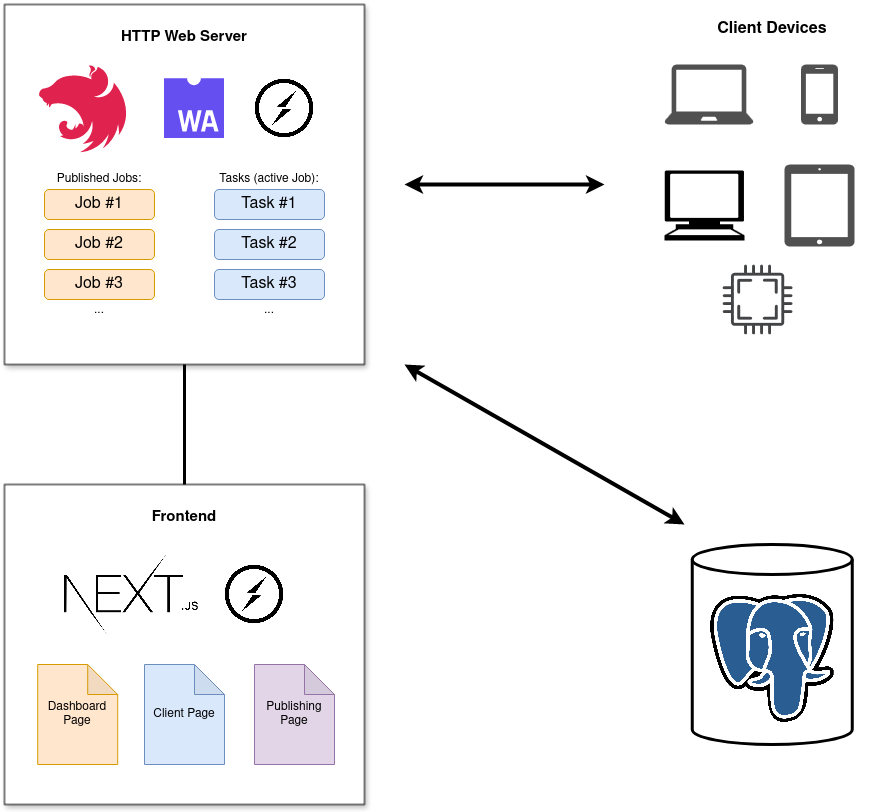
\includegraphics[width=0.95\textwidth]{gfx/figures/WebAssembly-MA.drawio.png}
    \caption{Architecture (Draft)}
    \label{fig:implementation:architecture}
\end{figure}

Figure \ref{fig:implementation:architecture} illustrates the architecture of the platform. Heterogenous clients, diverse in hardware or operating system, are able to connect to the platform. Each client (Worker and Administrator) is bidirectionally connected to the server through a WebSocket connection. The database is only accessible by the server.

\subsection{Communication}
\label{subsec:implementation:architecture:communication}
When a client connects to the platform by accessing the frontend application, a WebSocket connection is established to enable real-time and bidirectional communication. (TODO: Continue...)
\begin{figure}[htbp]
    \centering
    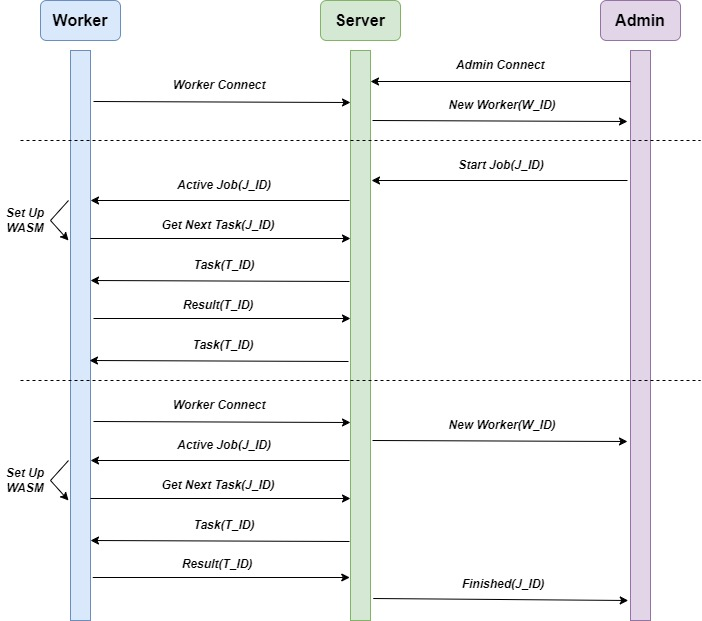
\includegraphics[width=0.95\textwidth]{gfx/figures/Communication.jpg}
    \caption{Communication (Draft)}
    \label{fig:implementation:architecture}
\end{figure}

\subsection{Persistence}
\label{subsec:implementation:architecture:persistence}


\subsubsection{Database}

\subsubsection{Task Input and Task Result}

\subsection{Scheduling}
\label{subsec:implementation:architecture:scheduling}


\section{Backend}
\label{sec:implementation:backend}
API endpoints 

\section{Frontend}
\label{sec:implementation:frontend}
Design and UI / Pages

\section{Security through Authentication}
\label{sec:implementation:authentication}
How can meliccious use can be prevented?

what is a JWT ? How is JWT used in this project? User vs Admin JWT

\section{Challenges}
\label{sec:implementation:challenges}
what was difficult?
\begin{itemize}
    \item Hadel Input and Output
    \item Output as File (PNG)
    \item Prevent dublicate Task execution
    \item Minimize Communication
\end{itemize}